\chapter{Predizione e osservazione dell'alta marea}
	In questo capitolo esamineremo il problema in cui la chiocciola osserva il momento d'inizio, di picco e di fine dell'alta marea e l'altezza raggiunta nel momento di picco di \textit{3 alte maree} consecutive che superino il livello del terreno, per poi fare una previsione sul momento di inizio, picco e fine della prossima alta marea, come dell'altezza raggiunta dal picco.\\
	Abbiamo quindi fissato il livello del terreno a \textbf{0.5}, dove 0 è il livello del mare in assenza di marea e 2 è il massimo picco di marea. Gli errori sui dati sensoriali corrispondono al \textbf{10\%} sulla percezione del livello di marea raggiunto ed un errore minimo, di massimo \textbf{5 minuti}, sullo scorrere del tempo.\\
	L'addestramento della rete, un Multilayer Perceptron, è avvenuto utilizzando \textit{500} pattern di esempio casuali, con relativi output obiettivo.\\
	\\
	Il risultato ottenuto è che il minimo numero di neuroni nello strato nascosto necessari per ottenere un errore medio di circa lo \textbf{0.1\%} risulta essere \textbf{17 neuroni}. Ancora una volta, quindi, si è arrivati alla conclusione che per effettuare una previsione del genere, anche se più complessa e anche in presenza di errori di percezione, la minima rete neurale necessaria risulta essere molto semplice. Per ottenere, invece, un errore medio inferiore all'\textbf{1\%} bastano \textbf{4 neuroni}, mentre per errori inferiori al \textbf{5\%} \textbf{2 neuroni} risultano essere sufficienti.\\
	Come ci si poteva aspettare da una previsione del genere, la rete simula molto meglio quando si hanno le 3 alte maree di osservazione e la marea da prevedere consecutive, ovvero 4 maree successive che superano il livello del terreno: infatti per questo tipo di predizione funzionano molto bene anche reti più semplici, anche con \textit{10 neuroni}. Tuttavia, specialmente nei periodi di \textit{neap tide}, ovvero quando si ha la luna in quadratura, le alte maree possono anche non riuscire a superare il livello del terreno e si possono avere anche giorni interi senza vedere la marea oppure vedendo una sola alta marea al giorno (al posto di due, come durante le \textit{spring tide}). In questi casi è richiesta appunto una rete neurale minimamente più complessa in quanto anche solo riuscire a predire dopo quanto tempo la marea riuscirà a superare nuovamente il livello del terreno è sicuramente un calcolo più complesso che calcolare il prossimo inizio di marea durante la spring tide (dove gli intervalli di tempo tra una marea e l'altra sono molto regolari).\\
	\\
	Di seguito vediamo alcuni grafici relativi a queste simulazioni: la funzione in blu rappresenta la funzione esatta di marea; la linea nera orizzontale indica il livello del terreno; i punti cerchiati in blu indicano l'osservazione dell'istante in cui è arrivata o finita la marea; i punti con un cerchio ed una X blu indicano i punti in cui si osserva l'arrivo e l'altezza del picco di marea; i punti cerchiati in rosso rappresentano la previsione sull'arrivo e fine della prossima alta marea; infine i punti con un cerchio ed una X rossa indicano la previsione fatta sul momento di arrivo e l'altezza del prossimo picco di marea.\\
	Per riprodurre queste simulazioni si veda il Codice \ref{lst:tideEdges}, Listato del codice.\\
	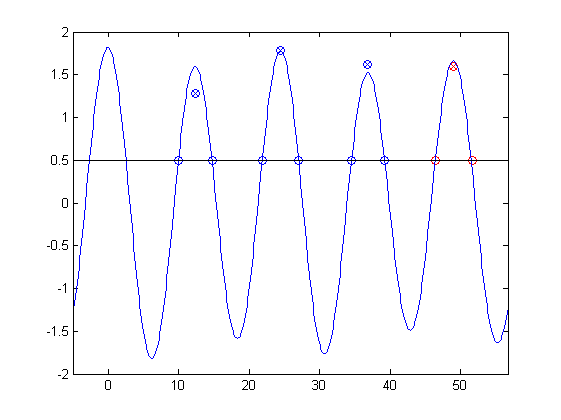
\includegraphics[width=0.6\textwidth]{edges_1.png}
	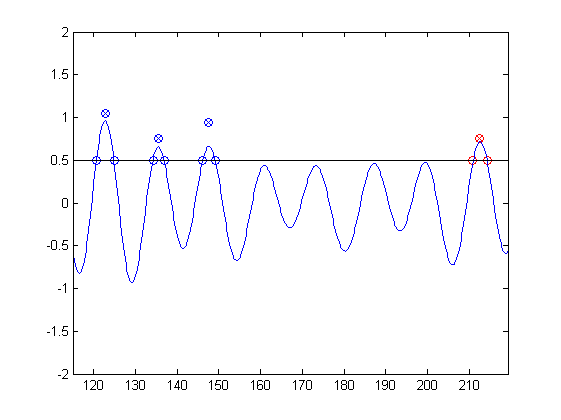
\includegraphics[width=0.6\textwidth]{edges_2.png}
	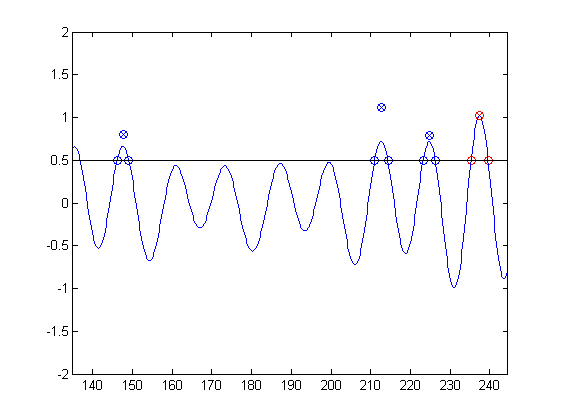
\includegraphics[width=0.6\textwidth]{edges_3.png}
	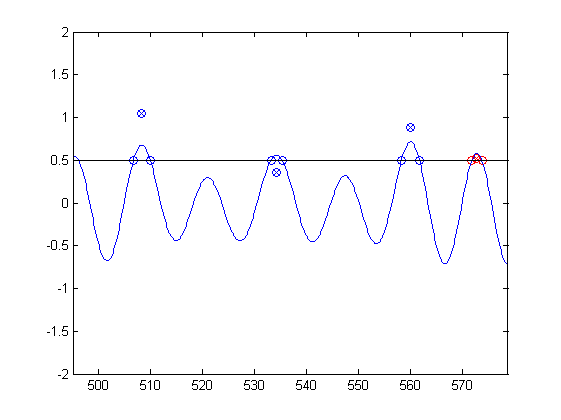
\includegraphics[width=0.6\textwidth]{edges_4.png}
	\FloatBarrier